\chapter{Analyse und Bewertung}
\label{chapter:evaluation}

\section{Einschränkende und Antreibende Faktoren}
\label{section:faktoren-change}

\paragraph{Einschränkende Faktoren der IT für Veränderungen}
\begin{enumerate}
    \item 
\end{enumerate}

\paragraph{antreibende Faktoren der IT für Veränderungsprozesse}
Die nachfolgenden antreibenden Faktoren betreffen die Fähigkeit der IT zur Umsetzung ihrer Veränderungs- oder \enquote{Change-} Prozesse. Diese sind nachfolgend mit einem allgemeinen Begriff aufgezählt und enthalten eine Analye und Bewertung. Die Auflistung ist anschließend sortiert nach der gegenseitigen Voraussetzung der Punkte. Ein genannter Punkt wird unter anderem für den Folgepunkt vorausgesetzt.

\begin{enumerate}
    \item \textbf{Offenheit \cite{Brockhoff2006}}
    
    \item \textbf{Zusammenarbeit}

    \item \textbf{Standardisierung} 
    
    Dieser Punkt umfasst Anwendungen, Systeme und Prozesse. Die Verwendung von gängigen sowie standardisierten Lösungen bringt eine Reihe von Vorteilen. Sie erhöht allen voran die Nachvollziehbarkeit der Systeme und sorgt für eine Effizienzsteigerung von Prozessen \cite{Strietzel2018, Bussmann2006, Alt2017}. 
    
    Beteiligte, insbesondere die Prüfer der Bankaufsicht und die interne Revision, können so mit einem Grundwissen über die IT die meisten Systeme auf Anhieb verstehen. Die Implementierung von \emph{Sicherheitstandards \cite{IT-Grundschutz:2020, Disterer2013}} ist hierbei besonders wichtig und bietet eine Grundlage für die Einhaltung der regulatorischen Vorgaben \cite{MaRisk:2017, BAIT:2018}.
    
    Der Einsatz von Standardsoftware führt zu einem effizienteren Ablauf in ihrer Wartung und Weiterentwicklung \cite{Bussmann2006}. Die Komplexität von operativen Systemen schränkt die Einführung von Standardsoftware jedoch ein \cite[S.27]{Bussmann2006}. Das Prinzip der \emph{Standardisierung} in Verbindung mit \emph{Offenheit} ergibt die Verwendung von \enquote{Open-Source} Software, die eine höhere Effizienzsteigerung aufgrund der Wiederverwendbarkeit der Komponenten bezweckt \cite{Brockhoff2006, Gupta:2017}. 
    
    Die Einführung von Standardsoftware hat ebenfalls Auswirkungen auf eingespielte Prozesse und die daraus folgenden Einzelentscheidungen beeinflussen in ihrer Summe die Entscheidung für oder gegen den Standard \cite[Tab.1]{Manz2018}.
    
    \item \textbf{Modularisierung}
    
    \item \textbf{Nachvollziehbarkeit}
    
    \item \textbf{Automatisierung}
    
    \item \textbf{Effizienzsteigerung}
    
    Die Effizienzsteigerung wirkt sich auf die verwendeten Ressourcen und Zeitaufwand der Prozesse, Systeme oder Anwendungen aus. Dazu zählen auch Kosten- und Personalaufwand. Es stellt sich die Frage in welchen Bereichen eine Effizienzsteigerung am sinnvollsten ist.
    
    Die Effizienzsteigerung wird vor allem im Bereich der Veränderungsprozesse \enquote{Change} bezüglich ihres Zeitaufwands erforderlich. Im Bereich der betrieblichen Prozesse \enquote{Run} ist sie primär für den Aufwand der Ressourcen erforderlich.
    
    Eine Effizienzsteigerung im Betrieb ermöglicht mehr Mittel für die \enquote{Change} Prozesse \cite{Rausch2006}. Dagegen steht das Prinzip, dass Ressourcen im Gegensatz zu Zeit finanziert und eingekauft werden können. Bevor an Opportunitäten in Form einer strategischen Weiterentwicklung der Produkte \cite{Rausch2006} gedacht wird, sollte die Weiterentwicklung der hierfür vorausgesetzten Veränderungsprozesse berücksichtigt werden. Die Fähigkeit für eine kontinuierliche Anpassung \cite{Bussmann2006, Ganswindt2006} der Produkte wird mit aktuellen Methoden, wie in Abb. \ref{fig:devops} dargestellt, bereits vorausgesetzt \cite{Alt2017}.

\end{enumerate}


\subsection{Digitale Transformation durch kontinuierliche Veränderungsprozesse}
 
Abb. \ref{fig:digit-trans} stellt für den Umgang mit Veränderungen ein erstes Prototyp dar.
 
An vielen Stellen sind die Symptome der Kreditinstitute bekannt (Kap. \ref{section:faktoren-change}). Hierfür ist die mangelnde Effizienz bei der Umsetzung von vorgenommenen Veränderungen die Ursache. Bis Organisationen auf Impulse reagieren und sich anpassen vergeht viel Zeit, die wichtigste Ressource der digitalen Transformation. Als Folge hierauf müssen Standardanwendungen aufwendig auf den überholten Zustand der Organisation angepasst werden. Änderungen werden in Folge an der falschen Stelle durchgeführt. 

Abb. \ref{fig:digit-trans} zeigt, dass die Antriebe und Einschränkungen erhebliche Einflüsse für die bevorstehende Transformation haben. Die Abbildung beschreibt die Startbedingungen einer bevorstehenden Transformation
Daher dient sie als Grundlage, um Anforderungen für einen innovationsorientierten Soll-Zustand der Organisation zu erzeugen.
Gleichzeitig zeigt sie, dass eine bevorstehende Transformation nur geregelt werden kann und die Auwirkungen nicht absehbar sind. Hierfür müssen Einschränkungen reduziert oder die Antriebe erhöht werden. Das Modell ist auf FinTechs und Start-ups übertragbar, da aufgrund einer größeren Risikoakzeptanz und geringerem Schutzbedarf ein einfacher Regelprozess ausreicht.

Für die größeren, etablierten Institute gilt ein erhöhter Schutzbedarf \cite{recht/Bornemann2018} und dadurch zusätzliche Maßnahmen für die Kontrolle von operationellen Risiken \cite{MaRisk:2017, BAIT:2018}.

Für den kontrollierten Umgang mit ständigen Veränderungen in der IT ist ein kontinuierlicher und effizienter Veränderungsprozess gefragt, womit die Transformation kontrollierbar stattfinden kann. Der Prototyp aus Abb. \ref{fig:digit-trans} muss daher in ein reiferes Modell verfeinert werden.
 
 \begin{figure}[htbp]
 \centering
 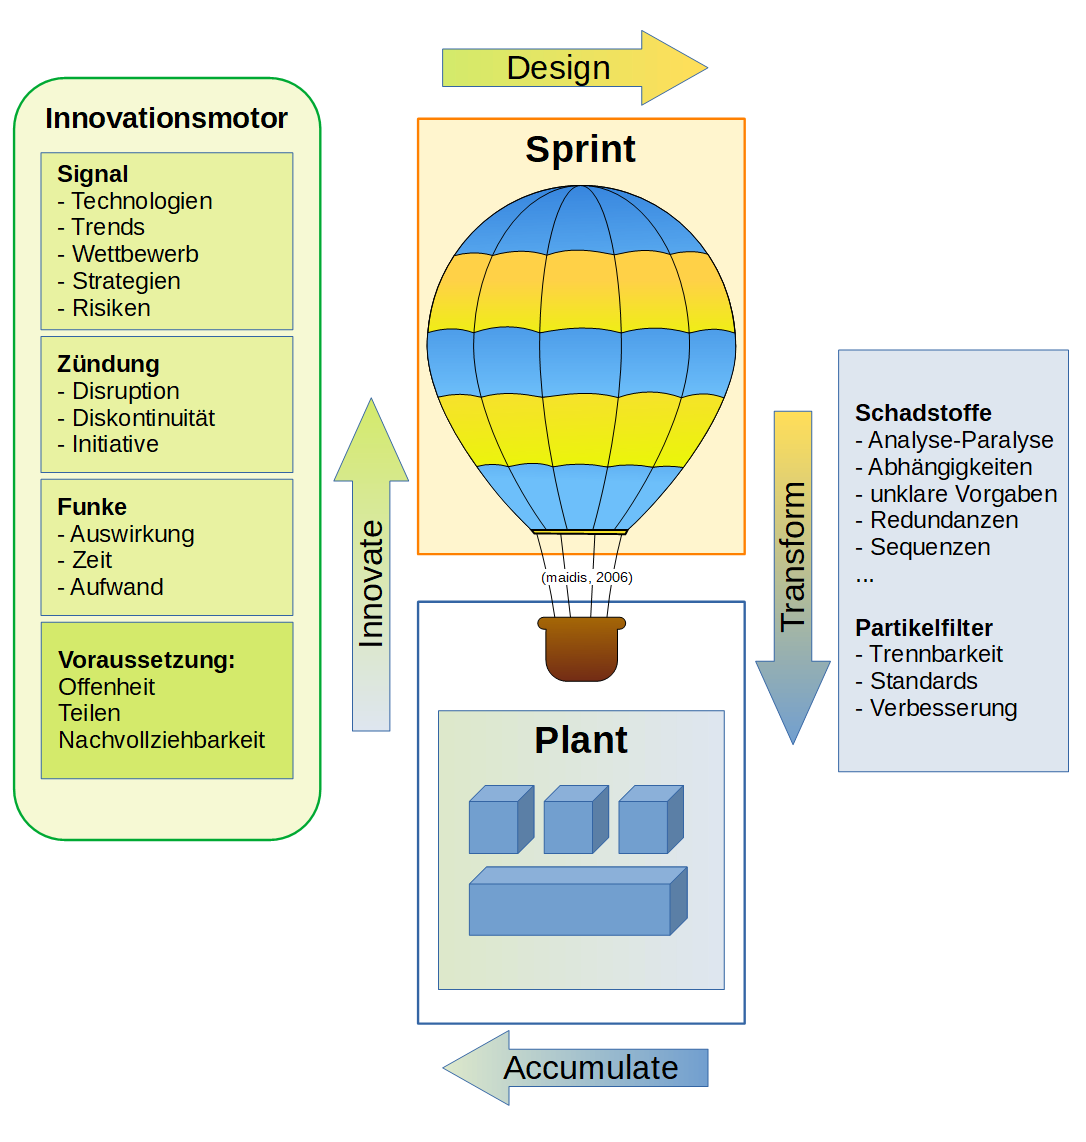
\includegraphics[width=1.0\textwidth]{gfx/digital-transformation-lifecycle-by-selim4.PNG}
 \caption{Transformations-Lebenszyklus: Kontinuierlicher Veränderungsprozess nach Innovate-Design-Transform inklusive Accumulate (Quelle: eigene Darstellung, Heißluftballon von \citet{maidis_2006})\label{fig:digit-trans-idt}
 }
 \end{figure}

\section{Zusammenfassung und Ausblick}
Es ergibt sich ein Gesamtbild, dass die aufgeführten Faktoren für Veränderungsprozesse keinen Ablauf oder direkte Handlungsempfehlungen beschreiben. Diese beschreiben \emph{Einflüsse} für Veränderungsprozesse und haben wesentliche Auswirkungen auf ihren Ablauf. Insbesondere die antreibenden Faktoren für Veränderungsprozesse können als ihre fachlichen Anforderungen gesehen werden. Prinzipien aus \emph{DevOps} und \emph{Design-Thinking} helfen dabei die Veränderungsprozesse selbst agil und kontinuierlich anzupassen. 

Darüber hinaus wird deutlich, dass die Informatik weitreichende Kompetenzen verfügt, aus dem Zusammenhang heraus auch Probleme aus anderen Bereichen zu lösen. Beginnend von der Ausgangssituation eines vorwiegend technischen Problems haben Lösungsansätze weitreichende Implikationen auf ihre nicht-technische Umgebung. Diese Implikationen bestätigen sich durch eine zunehmende Automatisierung von Geschäftsprozessen.

Kreative Methoden sind durch die Generierung von ad-hoc Zuständen in Form von Prototypen oder Beschreibungen wichtige Mittel in der Gestaltung von immateriellen Zuständen. Ihre Evaluierung ergibt sich aus der Koheränz zwischen Gegenwart, Risiken und Opportunität. Sie bieten keine direkt implementierbare Lösungen oder Handlungempfehlungen, sind aber für eine Strategie besonders wertvoll. Die steigende Kontinuität, Geschwindigkeit und Auswirkung von Veränderungen verlangen das Treffen von schnellen Entscheidungen, wofür Agilität in der Strategie bedingt wird. Geschieht dies nicht kann auch kein effizienter Veränderungsprozess entwickelt werden, welcher die in der Strategie definierten Ziele umsetzt. Mit ineffizienten Veränderungsprozessen entsteh Paralyse durch Analyse mit darauf folgender Handlungsunfähigkeit. 

Die einschränkenden Faktoren aus der IT-Architektur und Orgnisation spielen für ihre Transformation eine wichtige Rolle. Die Integration oder Inbetriebnahme von vorgenommenen Veränderungen in die Produktionsumgebung wird dadurch erschwert. 

Veränderungen bedingen reibungslose Veränderungsprozesse, welche die Transformation 


Die Komplexität

Darüber hinaus wird deutlich, dass die Informatik weitreichende Kompetenzen verfügt, aus dem Zusammenhang heraus auch Probleme aus anderen Bereichen zu lösen. Beginnend von der Ausgangssituation eines vorwiegend technischen Problems haben Lösungsansätze weitreichende Implikationen auf ihre nicht-technische Umgebung.

Kreative Methoden sind durch die Generierung von ad-hoc Zuständen in Form von Prototypen oder Beschreibungen wichtige Mittel in der Gestaltung von immateriellen Zuständen. Ihre Evaluierung ergibt sich aus der Koheränz zwischen Gegenwart, Risiken und Opportunität. Sie bieten keine direkten Lösungen oder Handlungempfehlungen, sind aber für deren Strategie besonders wertvoll. Die steigende Kontinuität, Geschwindigkeit und Auswirkung von Veränderungen verlangen das Treffen von schnellen Entscheidungen, wofür agilität in der Strategie beding wird.